\section{Implementácia}\label{sec:implementation}
Systém budeme implementovať v jazyku Python. Tento jazyk ponúka vhodné knižnice na prácu s konvolučnými sieťami a tiež na načítanie výstupu z našej kamery. Ku kamere výrobca vytvoril knižnicu s názvom `librealsense 2' v jazyku Python, ktorú používame na spracovanie údajov z kamery. Na vytvorenie konvolučnej neurónovej siete použijeme knižnicu `Keras'. Vytvoríme vlastný dataset a na jeho tvorbu napíšeme skript v jazyku Python s využitím vyššie spomínanej knižnice na načítanie obrázkov z kamery. Na vykreslenie obrázka v ktorom určíme súradnice použijeme knižnicu `openCV'.

\subsection{Vlastný dataset}
Prínosom pre predikciu súradníc v našom prostredí je doučiť sieť, ako vyzerá ruka v našom prostredí. Taktiež je vhodné na vstup do siete použiť rôzne polohy ruky. Na vytvorenie vlastného datasetu sme vytvorili skript v jazyku Python. Načítali sme dáta z kamery metódami knižnice `librealsense 2' a postupne sme prechádzali jednotlivými obrázkami z videa. Vybrali sme niekoľko scén a v nich zopár obrázkov zobrazujúcich reprezentatívne polohy rúk. Na načítaných obrázkoch sme ručne zvolili body so súradnicami predstavujúcimi kĺby, ktoré má sieť predikovať. Každý bod, na ktorý sme klikli uložil svoju polohu súradnicami $x, y$ tak, že bod $\left[0, 0\right]$ je v ľavom hornom rohu. Výhodou tohoto vlastného určovania pozície je, že sme súradnice ukladali vo forme, ktorú používame pri načítaní datasetu v našej sieti. Náš dataset obsahoval 100 obrázkov s označenými súradnicami kĺbov. Príklady polôh ruky v našom datasete sú znázornené na obr. \ref{img:our_hands}, kde sú červenými krúžkami označené nami určené súradnice. Tie však nie sú priamou súčasťou obrázka a vstup do siete je taký obrázok bez označenia súradníc.

\begin{figure}[H]
	\begin{center}
		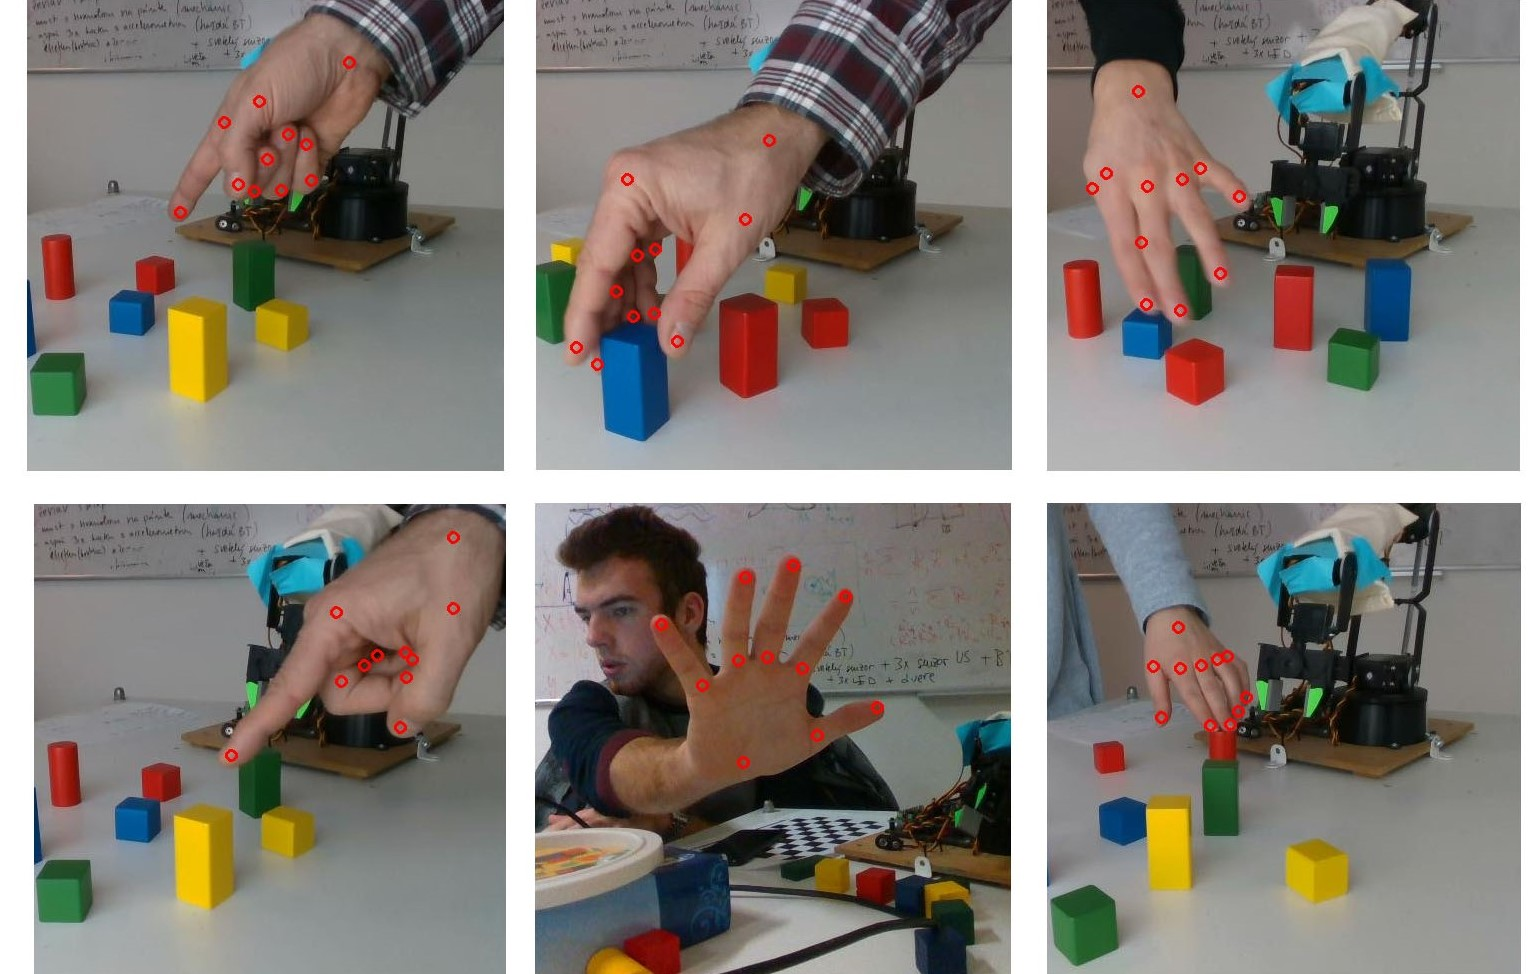
\includegraphics[width=\textwidth]{images/our_hands.jpg}
		\caption{Príklady obrázkov v našom  datasete.}
		\label{img:our_hands}
	\end{center}
\end{figure}

Štruktúru datasetu sme robili podľa vzoru NYUHands, aby sme pri dotrénovaní nášho datasetu zmenili iba cestu a nemuseli meniť kód. Názov obrázku sme zvolili s prefixom `rgb\_1\_', infix bol sedem miestne poradové číslo zhodné so súradnicami a sufixom `.jpg'. Súradnice sme ukladali do súboru vo formáte pre `MatLAB' ako štvorrozmerný tenzor (P, I, J, C). Pričom $P$ je index kamery (v našom prípade sme mali jednu, teda bol index 0), $I$ predstavuje index obrázka (určujúci obrázok príslušný k daným súradniciam), $J$ index kĺbu (určujúci pozície kĺbu) a $C$ súradnice $x, y$ príslušnému kĺbu.

\subsection{Predspracovanie}
Použili sme dáta z datasetu NYUhands ako vstup do našej siete a vybrali sme reprezentáciu obrázka v RGB. Tieto obrázky majú rozmer 640x480 pixlov a súradnice kĺbov tiež prislúchajú obrázkom vo forme u,v,d pre túto veľkosť. Keďže používame komplexnú sieť, je vhodné tieto dáta zmenšiť, aby sme urýchlili proces učenia a znížili nároky na veľkosť pamäte. 

Obrázky sme upravili tak, aby mali štvorcový rozmer a následne znížili rozlíšenie na 256x256. Poloha ruky na všetkých obrázkoch v datasete sa nachádza na ľavej časti obrázka, teda pri upravení na štvorcový rozmer sme odstránili 160 pixlov z pravej strany. Po tejto úprave nám zostali všetky súradnice kĺbov nezmenené, nakoľko súradnicová sústava má bod [0,0] v ľavom hornom rohu.

Navrhnutá sieť bude predikovať tepelné mapy. Očakávané súradnice sú v datasete reprezentovaný jedným bodom v obrázky. Preto sme na základe týchto súradníc vytvorili tepelné mapy. Na ich vytvorenie sme použili Gausovu distribúciu so stredom súradníc kĺbu a štandardnou odchýlkou 13 pixlov. Hodnotu štandardnej odchýlky sme empiricky hľadali tak, aby na vytvorenej tepelnej mape pokrývala dostatočnú časť okolia bodu. 

Tepelné mapy obsahujú hodnoty v intervale $\left[0, 1 \right]$, kde nenulová hodnota vyjadruje pozíciu kĺbu. Počas trénovania by teda rozdiel medzi tepelnou mapou a predikciou mapy obsahujúcej samé nuly bol veľmi malý. Preto sme každú hodnotu prenásobili hodnotou sto a teda vývoj chyby počas trénovania začal rádovo v stovkách nad nulou a klesal smerom k nule. 

\subsection{Architektúra siete}
Konvolučnú sieť sme zložili z dvoch reziduálnych častí, do ktorých vstupuje obrázok. Výstup prechádza cez poolingovú vrstvu do prvého modulu `Hourglass'. Zloženie vrstiev v tomto module popíšeme neskôr. Pripojili sme druhý takýto modul priamo za predošlí. Výstupom z druhého Hourglass modulu boli tepelné mapy, z ktorých sme vyberali súradnice kĺbov. Rozmery výstupu sú štyrikrát menšie, teda sme interpoláciou zväčšili ich rozmer na rozmer vstupných obrázkov. Táto architektúra je ilustračne znázornená na obr. \ref{img:our_architecture}. 

\begin{figure}[H]
	\begin{center}
		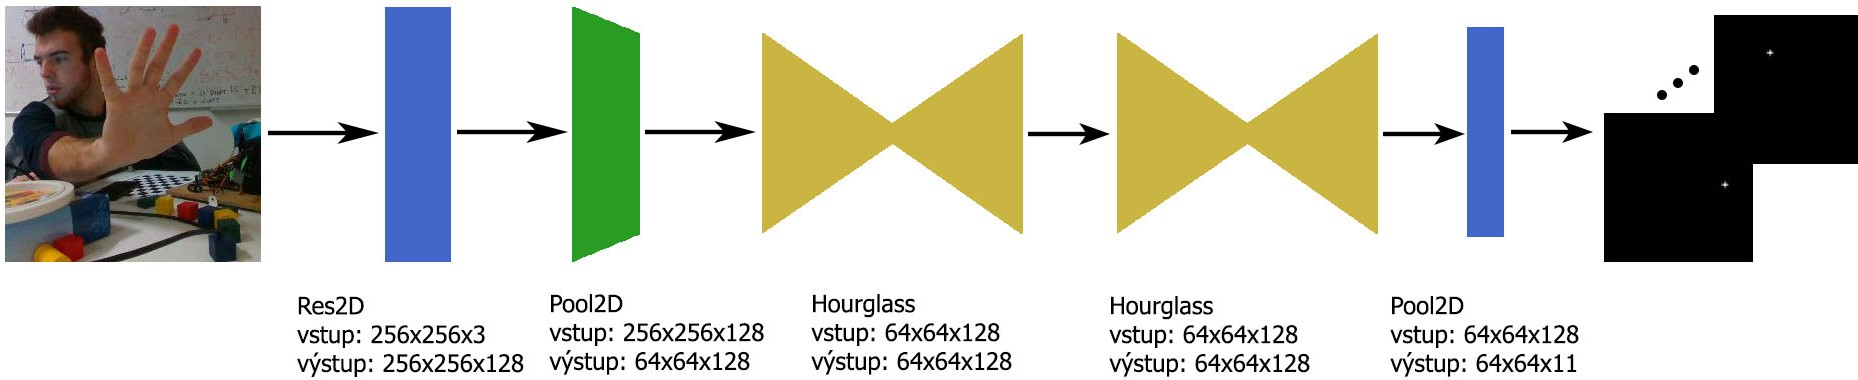
\includegraphics[width=\textwidth]{images/our_architecture.jpg}
		\caption{Architektúra siete, ktorú sme navrhli a implementovali. Vstupný obrázok je reprezentovaný maticou s rozmermi 256x256. Prvý blok vrstiev podvzorkuje za použitia poolingových vrstiev vstupnú maticu na rozmer 64x64. Tento ďalej vstupuje do modulu hourglass. Predikovaným výstupom je tepelná mapa s rozmerom 64x64 a ten ďalej upravíme časti úpravy výstupu.}
		\label{img:our_architecture}
	\end{center}
\end{figure}

\subsubsection{Hourglass implementácia}
Modul hourglass sme implementovali v jazyku Python a použili pri tom knižnicu Keras ako sme už spomínali aj v úvode kapitoly. Ako základ pre tento modul sme vychádzali podľa Newell a kol. \cite{DBLP:journals/corr/NewellYD16}, ktorý vytvorili tento modul pre predikovanie kostry človeka. 

V tejto architektúre sme využili reziduálne prepojenia (ich princíp sme ukázali v kapitole \ref{chap:issues_overview} odseku \ref{sec:residual}) také, že jedna vetva obsahuje konvolučnú vrstvu a vrstvu dávkovej normalizácie (nazývanú BatchNorm) trikrát za sebou a v druhej vetve nie je pridaná žiadna vrstva. Ilustrácia implementovaného reziduálneho prepojenia je na obr. \ref{img:42residual}. V časti zmenšovania vstupu sme použili pred každým reziduálnym prepojením poolingovú vrstvu s funkciou max. Takto sme zmenšovali vstup na polovicu po rozmer 8x8. Tu sme následne použili dve za sebou prepojení vyššie spomínané reziduálne prepojenia a ďalej sme pripravili časť zväčšovania. Výstup z vrstvy s menší rozmerom prešiel cez tzv. vrstvu UpSampling. Výstupom z nej bol rozmer dvojnásobný, teda rovnaký ako predchádzajúca vrstva. Matice na výstupe z týchto vrstiev boli sčítané a ich súčet bol upravený reziduálnym spojením. Tento postup sa opakoval až kým sme mali výstupný rozmer 64x64.

Posledné dve vrstvy, ktoré sme ešte pridali boli konvolučné s jadrom 1x1. Výstupná konvolučná vrstva mala počet filtrov rovnaký ako počet tepelných máp ktoré sme chceli predikovať. Tento počet sme implementovali konfigurovateľný, čo bolo vhodné pre testovanie a úpravu hyperparametrov. 

\begin{figure}[H]
	\begin{center}
		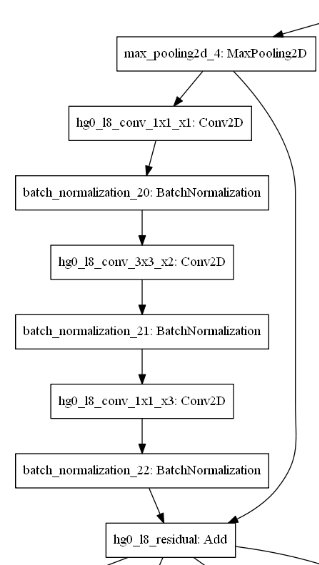
\includegraphics[height=250px]{images/42residual.png}
		\caption{Reziduálne prepojenie v module hourglass.}
		\label{img:42residual}
	\end{center}
\end{figure}

\subsection{Trénovanie}
Trénovanie sme rozdelili do dvoch častí. V prvej sme trénovali sieť na datasete NYUhands a v druhej časti sme použili natrénovanú sieť na nájdenie súradníc kĺbov pre obrázky vo vlastnom prostredí. Na spustenie trénovania takejto komplexnej siete je potrebný veľký hardvérový výkon. Využili sme službu `Google Cloud', kde sme vytvorili virtuálny počítač na serveroch od Google. 

Celý proces trénovania bol spustený na virtuálnom počítači. Aby sme mohli konzolové okno zavrieť a náš počítač vypnúť, vytvorili sme terminálovú reláciu pomocou príkazu `screen'. Vo vytvorenej relácii tak môže byť spustený proces a naša konzola môže byť zavretá. Taktiež sme potrebovali presunúť dataset na náš virtuálny počítač a natrénovaný model znovu späť na náš lokálny počítač. Na tieto presuny sme použili službu `bucket' v prostredí Google Cloudu. Virtuálnemu počítaču sme povolili zápis a čítanie na tento `bucket' a nástrojom `gsutil' sme presúvali súbory medzi `bucketom' a virtuálnym počítačom.

Sieť je veľmi citlivá na inicializáciu. Pri nevhodnom počiatočnom nastavení váh nie sieť schopná zlepšovať predikciu súradníc. Všetky vrstvy sme inicializovali Xavierovým \cite{glorot2010understanding} uniformným rozdelením. Trénovanie prebiehalo v troch fázach, pričom v každej z nich sme zvýšili počet tepelných máp, pre ktoré sme počítali chybu. Postupovali sme tak, že najprv sme počítali chybu pre konček palca. Po niekoľkých epochách, keď vedela sieť predikovať pozíciu končeka palca nad 60\%, pridali sme počítanie chyby pre všetky končeky prstov. Podobne ako v prvej fáze sme nechali trénovať sieť tak, aby každú mapu predikovala s presnosťou aspoň 60\%. V tretej fáze sme nastavili počítanie chyby pre všetky kĺby. Matematický výpočet chyby je popísaný rovnicou (\ref{eqn:euclideanLoss}). Pre každú fázu sme menili množinu M, ktorá obsahovala tepelné mapy príslušné k vyššie popísaným kĺbom. 

\subsubsection{Trénovanie na NYUHands}
Vstupné dáta sme rozdelili na trénovaciu množinu s 80\% obrázkov a validačnú množinu so zvyšnými 20\% obrázkov určenými na trénovanie. Stav siete je upravený metódou spätného šírenia chyby (popísanou v kapitole \ref{chap:issues_overview} v časti \ref{chpt:neuralNetwork}). Pre každý obrázok v trénovacej množine sa vypočíta chyba, teda rozdiel medzi predikovanými a očakávanými tepelnými mapami. Matematicky vyjadrené nasledujúcou rovnicou:

\begin{equation}\label{eqn:euclideanLoss}
    L2 = \sqrt{\sum_{b \in B, i \in H, j \in W, m \in M}{\left(y_{b,i,j,m} - \overset{\_}{y}_{b,i,j,h}\right)^{2}}}
\end{equation}

Kde B je množina obrázkov a k nim príslušným tepelných máp v jednej dávke. H označuje počet pixlov v stĺpci a W počet pixlov v riadku tepelnej mapy. M je množina tepelných máp pre obrázok b.

Spätné šírenie je pre dávku obrázkov. Veľkosť dávky je prínosná pre rýchlosť učenia siete. Množstvo obrázkov v sieti je potrebné vhodne zvoliť, pretože s jej zvyšujúcim počtom narastá požiadavka na veľkosť pamäte. Nastavili sme veľkosť dávky na 32 obrázkov, teda najväčšiu možnú veľkosť, ktorá sa ešte zmestí do pamäte počítača. 

Vypočíta sa priemerná hodnota zo všetkých chýb pre každý obrázok v dávke. Podľa nej sú potom upravené váhy v sieti. Takto sa postupuje pokiaľ sa vyhodnotia všetky obrázky v trénovacej množine. Tento postup nazývame priebeh epochy. Po každej epoche zistíme presnosť nášho modelu tak, že ako vstupné dáta zvolíme obrázky z validačnej množiny. V tejto časti trénovania sieť neupravuje hodnoty váh a slúži iba na vyhodnotenie kvality modelu.

\subsubsection{Dotrénovanie na vlastných dátach}
Inicializovali sme našu sieť váhami nastavenými podľa najlepšieho modelu, natrénovaného na datasete NYUhands. Výpočet chyby sme nastavili pre všetky kĺby podľa rovnice (\ref{eqn:euclideanLoss}). Vstupné dáta sme načítali z našej kamery a sieť sa učila lepšie predikovať súradnice kĺbov pre obrázky v našom prostredí.

\subsection{Vyhodnocovanie systému}
Pri vyhodnocovaní systému sme chceli sledovať presnosť určenia súradníc kĺbov ruky. Taktiež nás zaujímala presnosť jednotlivých kĺbov. Rozhodovací systém, či sú súradnice správne využíval prahovú hranicu, ktorá určovala maximálnu vzdialenosť medzi predikovanými a očakávanými súradnicami. Takto sme určili kružnicu s polomerom prahu a stredom v očakávaných súradniciach. Podobne ako v kapitole \ref{chap:previous_solutions} časti \ref{chpt:GANerated}, kde prahová hranica určovala priemer kruhu so stredom v očakávaných súradniciach, v ktorom sa musí predikovaný bod nachádzať, aby boli súradnice vyhodnotené ako správne. 

Sledovali sme dve prahové hranice nastavené na 2mm a 5mm pre určenie presnosti súradníc všetkých kĺbov a pre určenie presnosti každého kĺbu samostatne sme použili prahovú hranicu 5mm. Presnosť sme určovali v percentách ako pomer medzi správne určenými a všetkými súradnicami. 

Výpočet vzdialenosti bol ovplyvnený okrem predikcie aj zmenou veľkosti interpoláciou. Na minimalizovanie tejto chyby sme vydelili vypočítanú vzdialenosť konštantou, ktorú sme dostali nasledovným postupom. Tepelné mapy v pôvodnej veľkosti sme interpoláciou zmenšili na výstupný rozmer z našej siete (64x64). Tie sme spolu s príslušným obrázkom vložili na vstup pre určenie presnosti predikcie. Vedeli sme o správnosti všetkých kĺbov, a teda sme konštantu menili tak, aby systém vyhodnotil presnosť na 100\%.